% !TEX root = ../../main.tex
\chapter{Impact of Multijet Cut}
\label{ch:costhetastar}

As discussed in~\App{\ref{ch:qcd}}, a cut on the electron channel is introduced to suppress multijet background events which can be reconstructed as a mis-identified electron:
$$\frac{\MET}{\pt(W\rightarrow\ell\nu)} > 0.2$$
The cut effectively reduces the multijet background to less than $1$\,\%, including the previously problematic high-\pt region above $400$\,\GeV. The signal efficiency of the cut for the combined $e+\mu$ channel is 97\,\% for the HVT $Z'$ signal model for $m=2\,\TeV$\footnote{
	The cut is only included for the electron channel, which has a 93\,\% signal efficiency 
}. \Fig{\ref{fig:sens_mj}} illustrates the negligible impact of the cut on the sensitivity of the analysis.

\begin{figure}[htbp]
\begin{center}
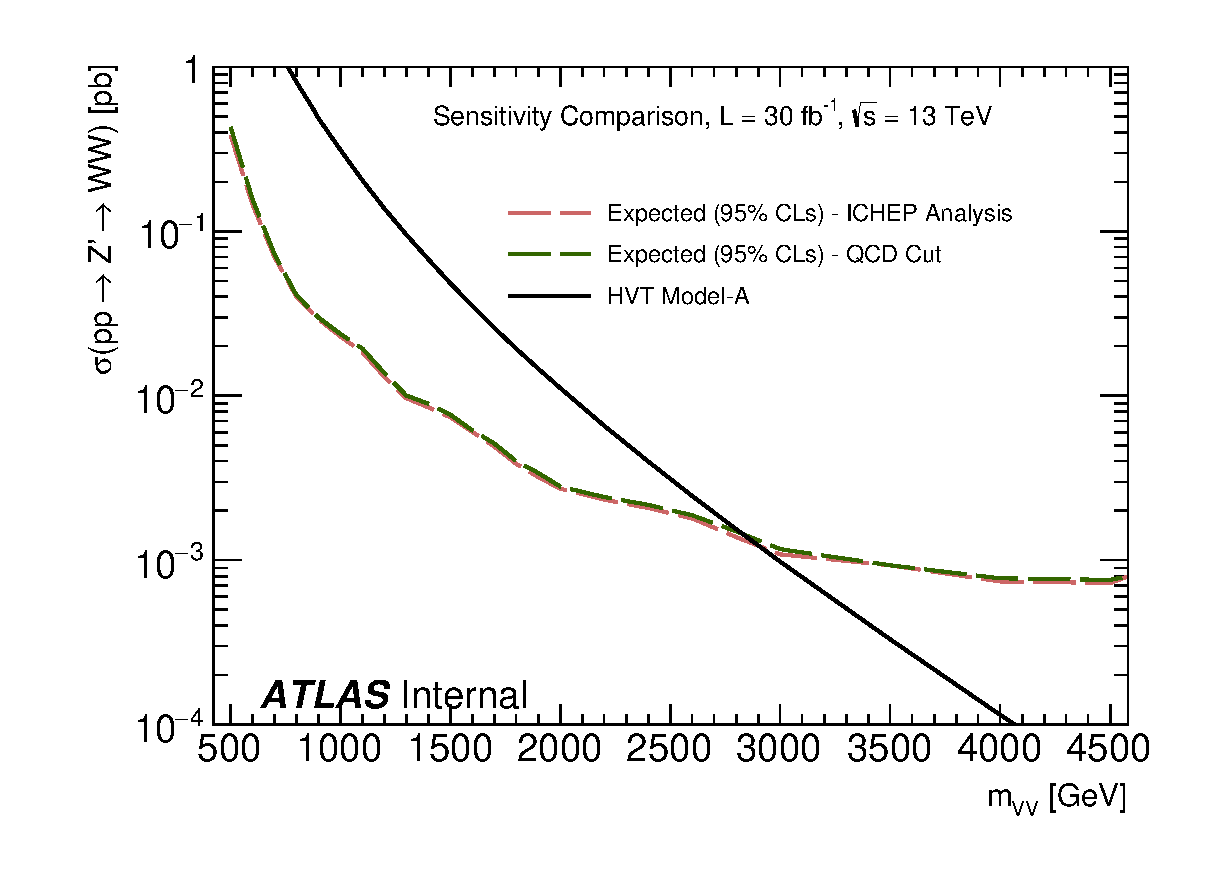
\includegraphics[width=0.7\textwidth]{figures/Appendix/sens_comparison}
\end{center}
\caption[Sensitivity comparison of multijet cut]{Projected sensitivity for 30\,\ifb with the nominal selection (red dotted line) and updated selection (green dotted line) which includes the multijet cut for the electron channel. The HVT $Z'\rightarrow WW$ Model-A interpretation is used. The multijet cut has a minimal impact on the projected sensitivity.}
\label{fig:sens_mj}
\end{figure}

%The Collis-Soper reference frame minimizes the smearing of $\cos\theta*$ due to initial \pt of the resonance, however the effect is expected to be small compared to the expected uncertainties.
Following the conventions laid out in \Ref{\cite{spin_parity}}, let $\theta_{e,W}$ be the polar angle between the electron and $W$ boson in the rest frame of the leptonically decaying $W$.
$$\cos\theta_{e,W} =  -\frac{\vec{q}_V\cdot\vec{q}_e}{|\vec{q}_V|\cdot|\vec{q}_e|}$$
Here, the three-momenta $\vec{q}_V, \vec{q}_e$ are defined in the $W$ rest frame, and $V$ corresponds to the hadronically decaying $W/Z$. As shown in \Fig{\ref{fig:costhetastar}}, the multijet cut removes events with $\cos\theta_{e,W}\sim1$\footnote{
	Events with small $\MET/\pt(W)$ tend to have the neutrino traveling backwards from the $W$ direction, while the electron is collinear. 
}.

The angular distributions of the electron from a left-handed, right-handed, and longitudinally polarized $W^{\pm}$ boson are
described by $(1\mp\cos\theta_{e,W})^2$  , $(1\pm\cos\theta_{e,W})^2$, and $\sin^2\theta_{eW}$, respectively~\cite{w_polarization}. The majority of $W$ bosons produced from scalar decays at high-\pt are longitudinally polarized~\cite{w_polarization_2}. Likewise, the $W'/Z'\rightarrow WV$ decay favors longitudinal polarization of the final state bosons in the limit of heavy $W'/Z'$ mass~\cite{hvt_polarization}\footnote{
	In this high $W'/Z'$ mass limit, the equivalence theorem indicates that the decay to longitudinal polarization states is enhanced as these modes become the goldstone bosons.
}. In the bulk RS graviton model, the localization of the Higgs field on the \TeV\,brane enhances the decay of the graviton to longitudinal weak bosons~\cite{rs_graviton}. \Fig{\ref{fig:costhetastar}} confirms this assertion for both $W^+$ and $W^-$ as their $\cos\theta_{e,W}$ distributions are mainly proportional to $\sin^2\theta_{e,W}$.
A high signal efficiency is thus expected. If there is a model which produces mainly right(left)-handed $W^+$($W^-$) bosons in the final state, the signal efficiency may be poor for the electron channel.
Since the cut is only applied for the electron channel, this signal model could still be observed by measuring an asymmetry between the electron and muon channels.

\begin{figure}[htbp]
\begin{center}
%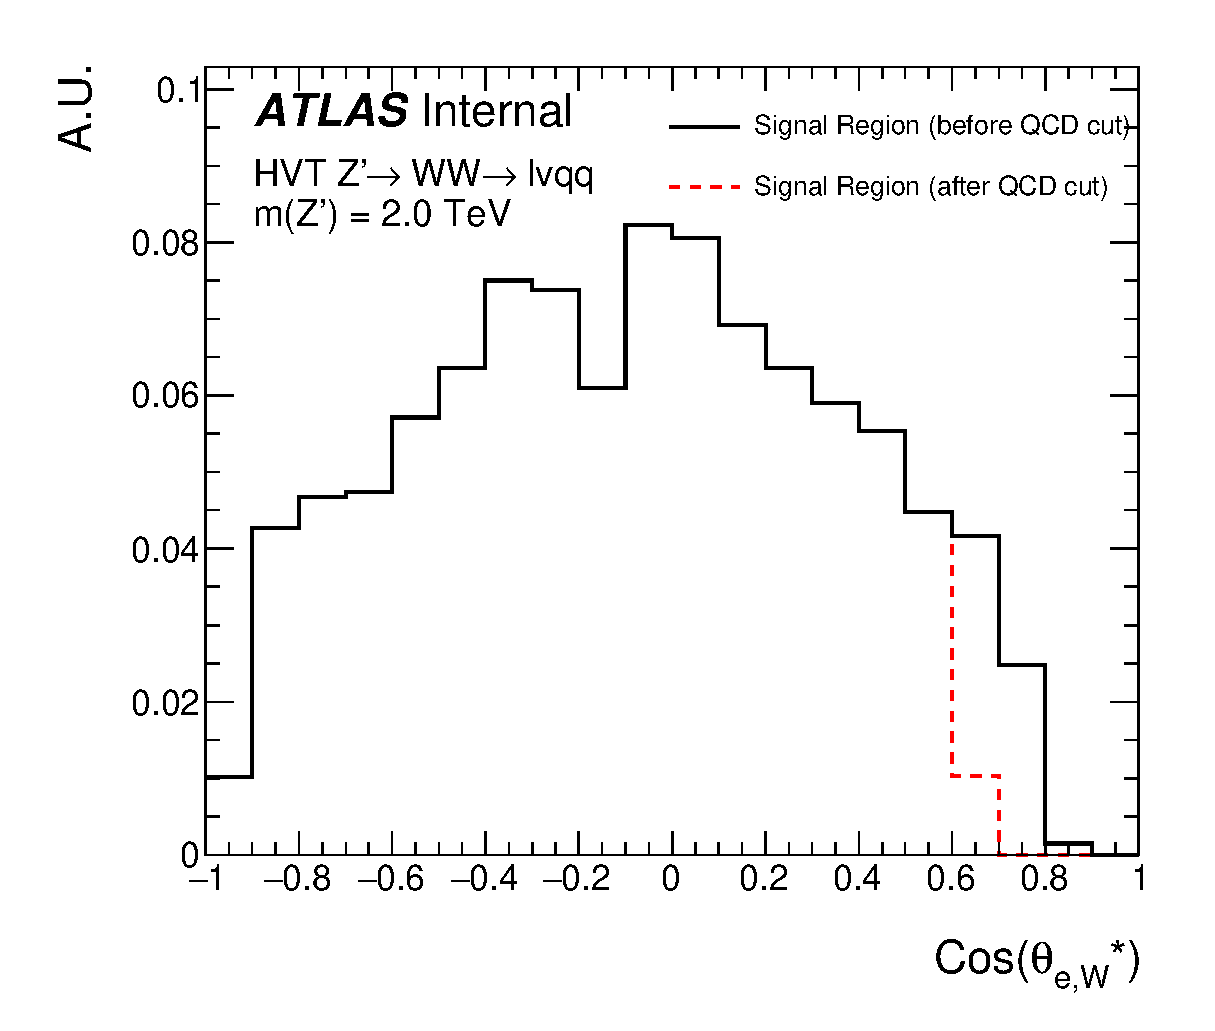
\includegraphics[width=.6\textwidth]{figures/Appendix/h_costhetastar}
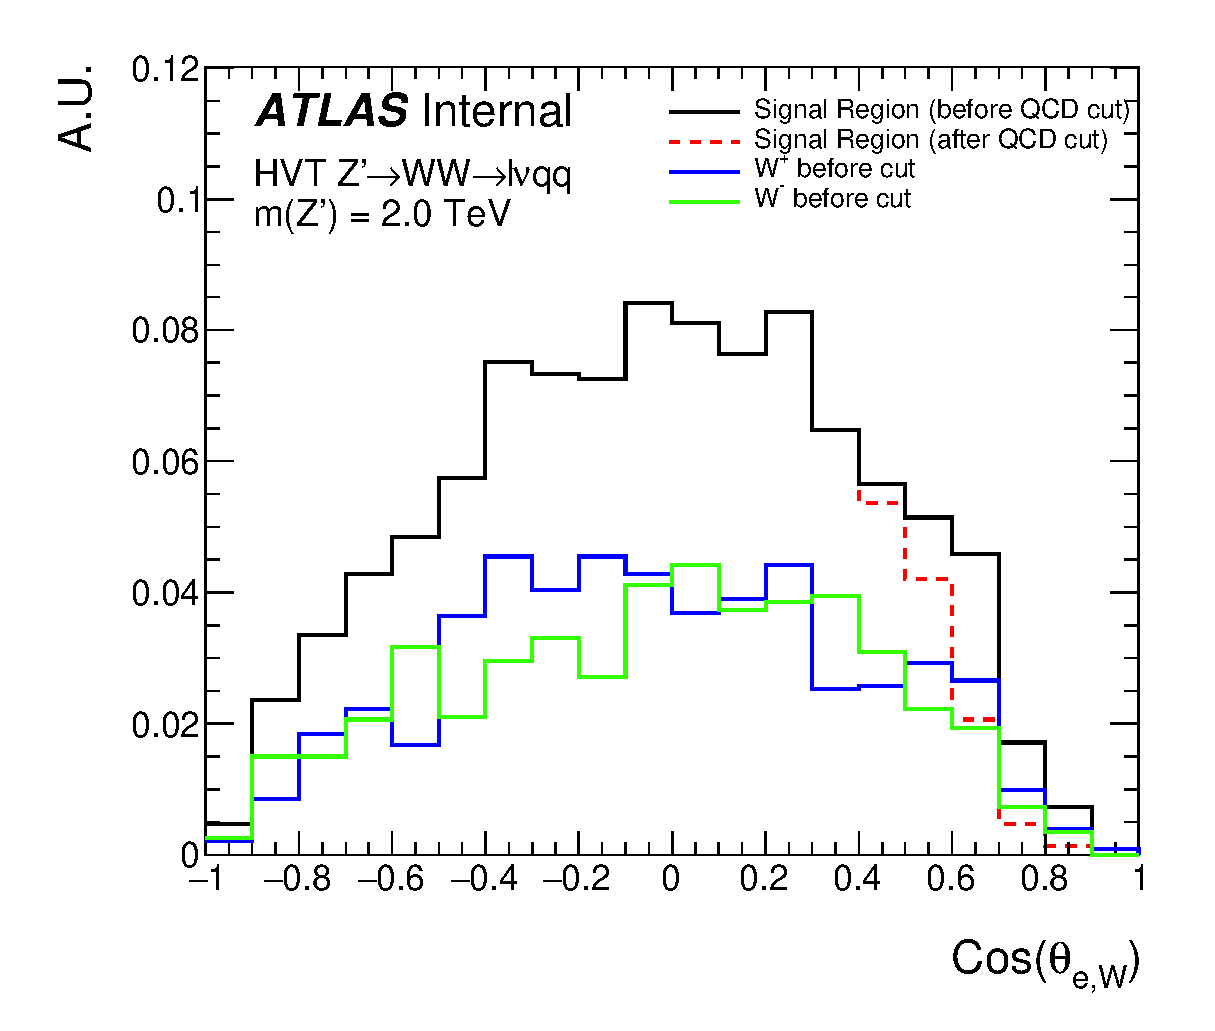
\includegraphics[width=.65\textwidth]{figures/Appendix/h_costhetastar_HVTWW}\\
\includegraphics[width=.65\textwidth]{figures/Appendix/h_costhetastar_VBFWW}
\end{center}
\caption[Cos$\theta_{e,W}$ between electron and W boson before and after QCD cut]{The $\cos\theta_{e,W}$ distribution in the signal region for the electron channel is shown before (black) and after (red dotted) a cut on $\MET/\pt$. The $W^+$ (blue) and $W-$ (green) distributions indicate a predominance of longitudinal polarization. An HVT $Z'\rightarrow WW$ (top) and VBF $H\rightarrow WW$ (bottom) signal sample is used for $m=2$\,\TeV. Most of the events cut are from the region $\cos\theta_{e,W}\sim1$, the $\mu$-channel can be used to detect an asymmetry.}
\label{fig:costhetastar}
\end{figure}

